\documentclass[11pt]{article}
\usepackage[margin=1in]{geometry}
\usepackage{amsmath,amssymb,amsthm,tikz,needspace}
\usepackage{tikz-cd}
\usetikzlibrary{arrows.meta,patterns}

\theoremstyle{definition}
\newtheorem{Def}{Definition}
\newtheorem{Ex}{Example}
\theoremstyle{remark}
\newtheorem{Rmk}{Remark}
\DeclareMathOperator{\ev}{ev}
\DeclareMathOperator{\Bl}{Bl}
\DeclareMathOperator{\ord}{ord}
\DeclareMathOperator{\divisor}{div}
\DeclareMathOperator{\Spec}{Spec}

\newcommand{\Sg}{\Sigma}
\newcommand{\sg}{\sigma}
\newcommand{\cO}{\mathcal{O}}
\newcommand{\set}[1]{\left\{#1\right\}}
\newcommand{\braket}[2]{\left\langle #1,#2\right\rangle}
\newcommand{\bA}{\mathbb{A}}
\newcommand{\bP}{\mathbb{P}}
\newcommand{\bR}{\mathbb{R}}
\newcommand{\bN}{\mathbb{N}}
\newcommand{\vf}{\varphi}
\newcommand{\x}{\times}
\newcommand{\isom}{\cong}

% Reuse the same schematic surface in diagrams 2 and 3.
\newcommand{\toricchart}{%
    \draw[gray!65,thick] (0.7,0) ellipse[x radius=2.45,y radius=1.35];
    \node at (2.6,1.2) {$X_\Sg$};
    \draw[teal!65!black,thick]
        (-1.55,0.18) .. controls (-1.12,0.72) and (-0.65,0.64) .. (-0.55,0.64)
        .. controls (0.12,0.46) and (1.02,0.52) .. (1.5,0.82)
        .. controls (1.66,0.91) and (1.8,1.02) .. (1.92,1.12);
    \draw[teal!65!black,thick]
        (-0.95,1.08) .. controls (-0.84,0.9) and (-0.72,0.77) .. (-0.55,0.64)
        .. controls (0.04,0.13) and (1.15,-0.01) .. (2.04,-0.49)
        .. controls (2.32,-0.65) and (2.54,-0.94) .. (2.55,-1.13);
    \draw[teal!65!black,thick]
        (1.19,1.11) .. controls (1.31,1.01) and (1.43,0.92) .. (1.5,0.82)
        .. controls (1.82,0.48) and (1.83,-0.07) .. (2.04,-0.49)
        .. controls (2.15,-0.71) and (2.23,-0.94) .. (2.26,-1.1);
    \foreach \point in {(-0.55,0.64),(1.5,0.82),(2.04,-0.49)}
        \fill \point circle (1.7pt);
    \draw[dashed,thick,gray] (-0.66,-0.02) ellipse[x radius=0.99,y radius=1.14];
    \node[below] at (-0.65,-1.18) {$X_\sigma$};
    \node[above left] at (-0.55,0.64) {$P_\sigma$};
    \node[below left,text=teal!65!black] at (-1.22,0.38) {$D_{\rho_1}$};
    \node[above left,text=teal!65!black] at (-0.95,1.08) {$D_{\rho_2}$};
}

\begin{document}

\begin{center}
    {\Large\bfseries October 16, 2026}
\end{center}

\section*{Recall from last time}

Let \(X_\Sg\) be a complete toric variety with character lattice \(M\),
and let
\[
    D=\sum_{\rho\in\Sg(1)}a_\rho D_\rho
\]
be a torus-invariant Cartier divisor. Its polytope is
\[
    P_D=\set{m\in M_\bR:\braket{m}{u_\rho}\geq-a_\rho
        \text{ for every }\rho\in\Sg(1)}.
\]
The lattice points of \(P_D\) index a basis of monomial global sections
of \(\cO_{X_\Sg}(D)\). When this set is nonempty, the complete linear
system defines a rational map
\[
    \vf_D:X_\Sg\dashrightarrow\bP^r,
    \qquad r=|P_D\cap M|-1.
\]
\begin{itemize}
    \item \(D\) is \emph{basepoint free} if its global sections have no
    common zero. The section formula then defines \(\vf_D\) everywhere.
    \item \(D\) is \emph{ample} if \(nD\) is very ample for some integer
    \(n>0\).
    \item \(D\) is \emph{very ample} if it is basepoint free and the
    induced morphism \(\vf_D\) is a closed embedding, identifying
    \(X_\Sg\) with its image in projective space.
\end{itemize}

\section{Basepoint-free divisors on toric varieties}

\subsection{Sections as rational functions}

Put \(L=\cO_{X_\Sg}(D)\). There is a distinguished rational section
\(s_D\) with \(\divisor(s_D)=D\). It need not be regular when \(D\)
has negative coefficients. Every other nonzero rational section can be written
uniquely as
\[
    \widetilde{s}=f s_D,
    \qquad f=\frac{\widetilde{s}}{s_D},
\]
and
\[
    \divisor(\widetilde{s})=\divisor(f)+D.
\]
To test basepoint freeness at \(P\), we ask whether there is a
\emph{global regular} section \(\widetilde{s}\) with
\(\widetilde{s}(P)\neq0\).

\Needspace{6cm}
\begin{center}
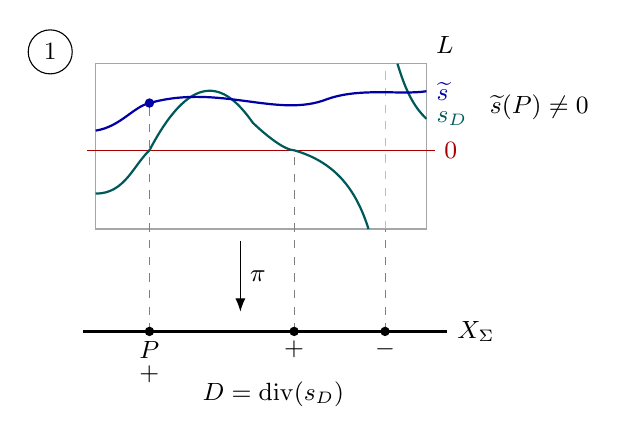
\begin{tikzpicture}[x=1.05cm,y=1cm,>=Latex,every node/.style={font=\small}]
    \node[draw,circle,inner sep=3pt] at (-0.55,3.55) {$1$};
    \draw[gray!70] (0,1.3) rectangle (4,3.4);
    \node[above right] at (4,3.4) {$L$};
    \draw[red!65!black] (-0.1,2.3) -- (4.1,2.3) node[right] {$0$};
    % A schematic meromorphic section: two zeros and a pole.
    \draw[teal!70!black,thick] (0,1.75)
        .. controls (0.35,1.75) and (0.45,2.1) .. (0.65,2.3)
        .. controls (1.2,3.4) and (1.6,3.1) .. (1.9,2.65)
        .. controls (2.1,2.45) and (2.3,2.3) .. (2.4,2.3)
        .. controls (2.9,2.15) and (3.15,1.8) .. (3.3,1.3);
    \draw[teal!70!black,thick] (3.65,3.4)
        .. controls (3.75,3.05) and (3.85,2.85) .. (4,2.7)
        node[right] {$s_D$};
    \draw[dashed,teal!40] (3.5,1.3) -- (3.5,3.4);
    \draw[blue!65!black,thick] (0,2.55)
        .. controls (0.3,2.6) and (0.45,2.85) .. (0.65,2.9)
        .. controls (1.5,3.15) and (2.2,2.7) .. (2.8,2.95)
        .. controls (3.2,3.1) and (3.7,3.0) .. (4,3.05)
        node[right] {$\widetilde{s}$};
    \draw[thick] (-0.15,0) -- (4.25,0) node[right] {$X_\Sg$};
    \draw[dashed,gray] (0.65,0) -- (0.65,2.9);
    \draw[dashed,gray] (2.4,0) -- (2.4,2.3);
    \draw[dashed,gray] (3.5,0) -- (3.5,1.3);
    \fill (0.65,0) circle (1.7pt) node[below] {$P$};
    \fill (2.4,0) circle (1.7pt) node[below] {$+$};
    \fill (3.5,0) circle (1.7pt) node[below] {$-$};
    \node at (0.65,-0.55) {$+$};
    \fill[blue!65!black] (0.65,2.9) circle (1.7pt);
    \draw[->] (1.75,1.15) -- (1.75,0.25) node[midway,right] {$\pi$};
    \node[right] at (4.65,2.85) {$\widetilde{s}(P)\ne0$};
    \node at (2.15,-0.8) {$D=\divisor(s_D)$};
\end{tikzpicture}

{\small Schematic curve picture: positive coefficients record zeros of
\(s_D\), and negative coefficients record poles.}
\end{center}

On a smooth curve, write \(a_P=\ord_P(s_D)\). For a regular section,
\[
    \widetilde{s}(P)\ne0
    \quad\Longleftrightarrow\quad
    \ord_P(f)=-a_P.
\]
Thus a zero of order \(a_P>0\) must be cancelled by a pole of that
order in \(f\), and a pole of \(s_D\) must be cancelled by a zero of
\(f\). The orders need not be one. In higher dimensions, divisor
orders are taken along prime divisors rather than at arbitrary points.

\subsection{Torus eigensections and affine charts}

The torus action lets us work with eigensections
\[
    s_m=\chi^m s_D,\qquad m\in M.
\]
Since a character has zeros and poles only along the toric boundary,
\[
    \divisor(s_m)=\sum_{\rho\in\Sg(1)}
        \bigl(\braket{m}{u_\rho}+a_\rho\bigr)D_\rho.
\]
Consequently,
\[
    s_m\text{ is globally regular}
    \quad\Longleftrightarrow\quad
    m\in P_D\cap M.
\]
Every global regular section is a linear combination of these
eigensections. The rational function \(\chi^m\) may have poles even
when the section \(s_m\) is regular: its poles are allowed to cancel
the positive part of \(D\).

Let \(\sigma\) be a full-dimensional maximal cone, and write
\[
    X_\sigma=\Spec k[\sigma^\vee\cap M].
\]
This affine chart has a distinguished torus-fixed point \(P_\sigma\),
the closed orbit corresponding to \(\sigma\). Every invariant divisor
\(D_\rho\) with \(\rho\in\sigma(1)\) passes through \(P_\sigma\).
These are exactly the invariant boundary divisors meeting the chart.

\Needspace{4cm}
\begin{center}
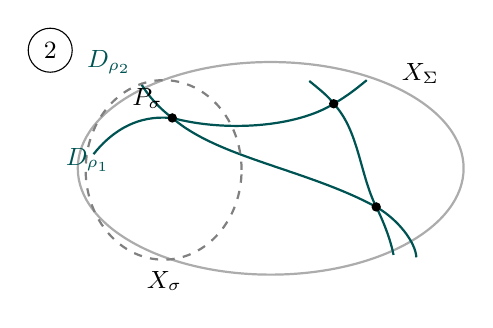
\begin{tikzpicture}[>=Latex,every node/.style={font=\small}]
    \node[draw,circle,inner sep=3pt] at (-2.1,1.5) {$2$};
    \toricchart
\end{tikzpicture}

{\small The toric boundary, its fixed points, and the affine chart
\(X_\sigma\) (schematic).}
\end{center}

\subsection{The section that does not vanish at \(P_\sigma\)}

Because \(D\) is Cartier, there is an integral vector \(m_\sigma\in M\)
such that
\[
    \braket{m_\sigma}{u_\rho}=-a_\rho
    \qquad\text{for every }\rho\in\sigma(1).
\]
The Cartier condition guarantees existence, even if the cone is not
simplicial; full dimension guarantees uniqueness. The local equation
and the corresponding local frame of \(L\) are
\[
    g_\sigma=\chi^{-m_\sigma},\qquad
    D|_{X_\sigma}=\divisor(g_\sigma),\qquad
    e_\sigma=g_\sigma^{-1}s_D=\chi^{m_\sigma}s_D.
\]
The frame \(e_\sigma\) is regular and nowhere zero on \(X_\sigma\).
An eigensection has local expression
\[
    s_m=\chi^{m-m_\sigma}e_\sigma.
\]
If \(s_m\) is regular on this chart, then
\(m-m_\sigma\in\sigma^\vee\cap M\). At \(P_\sigma\), every nonconstant
regular monomial vanishes. Since \(\sigma\) is full dimensional,
\[
    \boxed{s_m(P_\sigma)\ne0\quad\Longleftrightarrow\quad m=m_\sigma.}
\]
Equivalently, a regular eigensection is nonzero there precisely when
\[
    \braket{m}{u_\rho}=-a_\rho
    \qquad\text{for all }\rho\in\sigma(1).
\]
Such a section trivializes \(L\) on the entire affine chart.

\begin{Rmk}
    The eigensection hypothesis matters. A general regular section
    nonzero at the fixed point need not be nowhere zero on the chart:
    \(1+x\) on \(\bA^1\) is nonzero at \(0\) but vanishes at \(-1\).
    Also, vanishing orders along the boundary alone do not detect
    nonvanishing of an arbitrary section at a fixed point: \(x+y\)
    vanishes at the origin but has order zero along both coordinate axes.
\end{Rmk}

\subsection{The local model \(x^2/y\)}

\begin{Ex}
    Suppose \(X_\sigma\cong\bA^2\) is a smooth surface chart with
    \(D_{\rho_1}=V(x)\) and \(D_{\rho_2}=V(y)\). Take
    \[
        D|_{X_\sigma}=2V(x)-V(y)=\divisor\!\left(\frac{x^2}{y}\right).
    \]
    Thus the distinguished rational section has a zero of order two
    along \(V(x)\) and a pole of order one along \(V(y)\).

    \Needspace{7cm}
    \begin{center}
    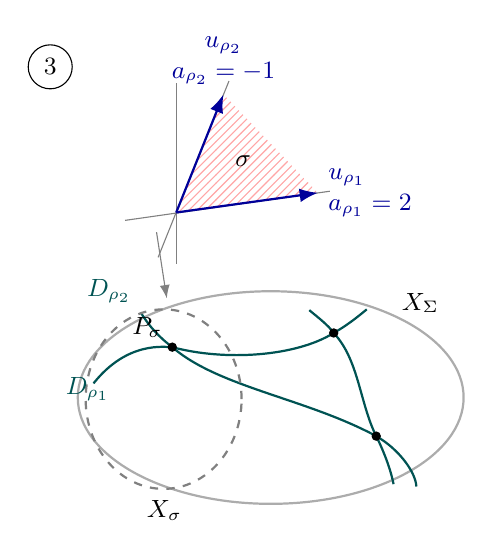
\begin{tikzpicture}[>=Latex,every node/.style={font=\small}]
        \node[draw,circle,inner sep=3pt] at (-2.1,4.2) {$3$};
        \toricchart
        \begin{scope}[shift={(-0.5,2.35)}]
            \path[pattern=north east lines,pattern color=red!35]
                (0,0) -- (1.8,0.25) -- (0.6,1.5) -- cycle;
            \draw[gray] (-0.65,-0.1) -- (1.95,0.27);
            \draw[gray] (-0.23,-0.57) -- (0.67,1.67);
            \draw[gray] (0,-0.65) -- (0,1.65);
            \draw[->,blue!60!black,thick] (0,0) -- (1.8,0.25)
                node[right,align=left] {$u_{\rho_1}$\\$a_{\rho_1}=2$};
            \draw[->,blue!60!black,thick] (0,0) -- (0.6,1.5)
                node[above,align=center] {$u_{\rho_2}$\\$a_{\rho_2}=-1$};
            \node at (0.85,0.65) {$\sigma$};
        \end{scope}
        \draw[->,gray] (-0.75,2.1) -- (-0.62,1.26);
    \end{tikzpicture}

    {\small The cone \(\sigma\), its divisor coefficients, and its
    corresponding affine chart.}
    \end{center}

    With respect to the dual basis determined by \(x,y\),
    \[
        m_\sigma=(-2,1),\qquad
        e_\sigma=\frac{y}{x^2}s_D.
    \]
    Write a regular section on the chart as
    \(\widetilde{s}=p(x,y)e_\sigma\), where \(p(x,y)\) is a polynomial.
    Its associated rational function is
    \[
        f=\frac{\widetilde{s}}{s_D}
          =p(x,y)\frac{y}{x^2}.
    \]
    We have \(\widetilde{s}(P_\sigma)\ne0\) exactly when
    \(p(0,0)\ne0\). In that case,
    \[
        \ord_{V(x)}(f)=-2,\qquad \ord_{V(y)}(f)=1.
    \]
    The eigensection corresponding to \(p=1\) is the local frame
    \(e_\sigma=s_{m_\sigma}\). Its extension to a global section is
    determined by the remaining inequalities defining \(P_D\).
\end{Ex}

\subsection{The global basepoint-free criterion}

For each maximal cone, the Cartier datum \(m_\sigma\) gives the only
possible exponent of an eigensection nonzero at \(P_\sigma\). This
candidate extends to a global regular section exactly when
\[
    m_\sigma\in P_D,
    \quad\text{that is,}\quad
    \braket{m_\sigma}{u_\rho}\geq-a_\rho
    \quad\text{for every }\rho\in\Sg(1).
\]
The rays of \(\sigma\) impose equalities; rays outside \(\sigma\)
give the additional tests for global regularity.

If a global regular section is nonzero at \(P_\sigma\), one of its
monomial summands must also be nonzero there. That summand has exponent
\(m_\sigma\), so \(m_\sigma\in P_D\). Conversely, if
\(m_\sigma\in P_D\), the global section \(s_{m_\sigma}\) is a frame
on \(X_\sigma\). Since these charts cover \(X_\Sg\),
\[
    \boxed{D\text{ is basepoint free}
    \quad\Longleftrightarrow\quad
    m_\sigma\in P_D\text{ for every maximal cone }\sigma.}
\]

\begin{Rmk}[The sign convention]
    Here \(m_\sigma\) is the exponent of the local frame, so
    \(\braket{m_\sigma}{u_\rho}=-a_\rho\). If instead the Cartier
    data are written as exponents \(q_\sigma\) of the local defining
    equations, then \(q_\sigma=-m_\sigma\), and the same criterion
    reads \(-q_\sigma\in P_D\). The minus sign comes from taking the
    reciprocal of the local defining equation to obtain a frame.
\end{Rmk}

\subsection{Reading regularity from the half-spaces}

Each ray \(\rho\) determines a half-space in the character space
\(M_\bR\):
\[
    H_\rho=\set{m\in M_\bR:\braket{m}{u_\rho}\geq-a_\rho},
    \qquad P_D=\bigcap_{\rho\in\Sg(1)}H_\rho.
\]
For a full-dimensional cone \(\sigma\), the boundary hyperplanes
associated to its rays meet at the Cartier datum \(m_\sigma\).
These equalities guarantee a local frame on \(X_\sigma\). To extend
that frame globally, \(m_\sigma\) must also lie in every remaining
half-space. Thus it is the section \(s_{m_\sigma}\), rather than the
lattice vector itself, whose global regularity we are testing.

The following model keeps the two local conditions \(r,t\geq0\) and
their intersection \(m_\sigma=(0,0)\) fixed. The other two conditions
are \(t-r\geq c\) and \(t\leq3\), so
\[
    P_c=\set{(r,t):r\geq0,\ t\geq0,\ t-r\geq c,\ t\leq3}.
\]
These inequalities come from the complete fan with rays
\((1,0)\), \((0,1)\), \((-1,1)\), and \((0,-1)\).
Changing \(c\) changes one divisor coefficient without changing
\(m_\sigma\).

\Needspace{7cm}
\begin{center}
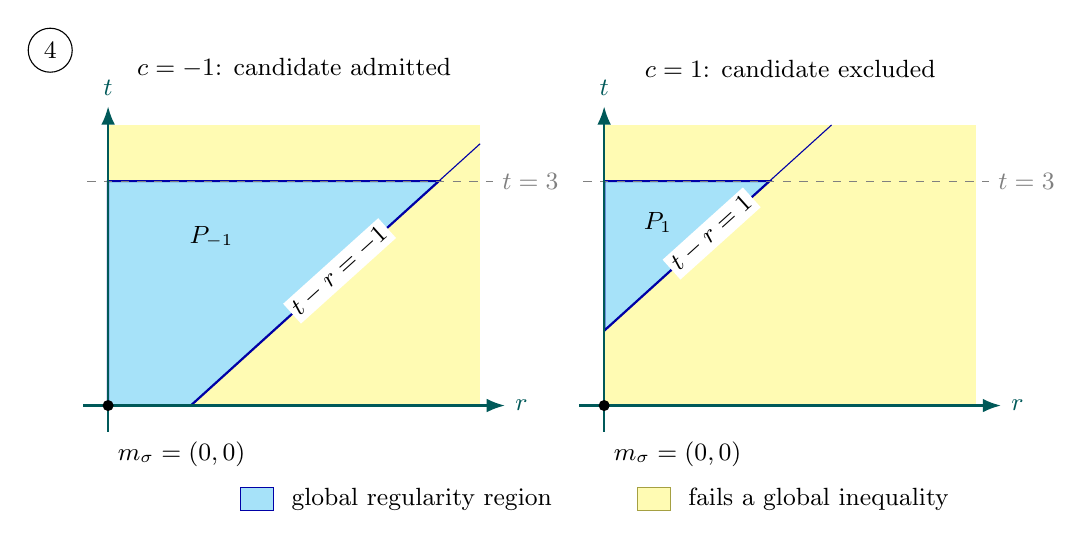
\begin{tikzpicture}[
    x=1.05cm,y=0.95cm,>=Latex,
    every node/.style={font=\small}
]
    \node[draw,circle,inner sep=3pt] at (-0.7,4.75) {$4$};
    \foreach \offset/\case in {0/1,6.3/2} {
        \begin{scope}[xshift=\offset cm]
            % Yellow consists of local candidates outside the polytope.
            \fill[yellow!30] (0,0) rectangle (4.5,3.75);
            \ifnum\case=1
                \fill[cyan!35] (0,0) -- (1,0) -- (4,3) -- (0,3) -- cycle;
                \draw[thick,blue!65!black]
                    (0,0) -- (1,0) -- (4,3) -- (0,3) -- cycle;
                \draw[blue!65!black] (1,0) -- (4.5,3.5);
                \node[above] at (2.25,4.25) {$c=-1$: candidate admitted};
                \node[fill=white,inner sep=1.5pt,rotate=42]
                    at (2.8,1.8) {$t-r=-1$};
                \node at (1.25,2.25) {$P_{-1}$};
            \else
                \fill[cyan!35] (0,1) -- (2,3) -- (0,3) -- cycle;
                \draw[thick,blue!65!black]
                    (0,1) -- (2,3) -- (0,3) -- cycle;
                \draw[blue!65!black] (0,1) -- (2.75,3.75);
                \node[above] at (2.25,4.25) {$c=1$: candidate excluded};
                \node[fill=white,inner sep=1.5pt,rotate=42]
                    at (1.3,2.3) {$t-r=1$};
                \node at (0.65,2.45) {$P_1$};
            \fi
            \draw[dashed,gray] (-0.25,3) -- (4.65,3)
                node[right] {$t=3$};
            \draw[->,teal!70!black,thick] (-0.3,0) -- (4.8,0)
                node[right] {$r$};
            \draw[->,teal!70!black,thick] (0,-0.35) -- (0,4.0)
                node[above] {$t$};
            \fill[black] (0,0) circle (2pt);
            \node[below right] at (0,-0.35) {$m_\sigma=(0,0)$};
        \end{scope}
    }
    \fill[cyan!35,draw=blue!65!black] (1.6,-1.4) rectangle (2,-1.1);
    \node[right] at (2.1,-1.25) {global regularity region};
    \fill[yellow!30,draw=yellow!60!black] (6.4,-1.4) rectangle (6.8,-1.1);
    \node[right] at (6.9,-1.25) {fails a global inequality};
\end{tikzpicture}
\end{center}

Blue is the polytope whose lattice points index globally regular
eigensections. Yellow lies in the local cone of candidates but outside the polytope.
In the left panel, \(m_\sigma\in P_{-1}\), so its section extends
globally. In the right panel, \(m_\sigma\notin P_1\), so it does not.
The blue region is still nonempty there: other global sections exist,
but all vanish at \(P_\sigma\).

\subsection{From Cartier data to a convex support function}

To match the convention used on the board, write
\(q_\sigma=-m_\sigma\) for the exponent of the local defining equation.
Define the piecewise-linear function \(\psi_D:N_\bR\to\bR\) by
\[
    \psi_D(u)=\braket{q_\sigma}{u}
    \quad\text{for }u\in\sigma.
\]
The Cartier compatibility conditions make these linear functions agree
on common faces, so \(\psi_D\) is continuous. On the primitive ray
generators,
\[
    \psi_D(u_\rho)=a_\rho.
\]
The global regularity condition becomes
\[
    m_\sigma=-q_\sigma\in P_D
    \quad\Longleftrightarrow\quad
    \braket{q_\sigma}{u_\rho}\leq a_\rho
    \quad\text{for every }\rho\in\Sg(1).
\]

Suppose these inequalities hold for every maximal cone \(\sigma\).
Fix one of its linear functions \(\braket{q_\sigma}{\cdot}\).
On any other cone \(\tau\), the ray inequalities and linearity give
\[
    \braket{q_\sigma}{u}\leq\psi_D(u)
    \qquad(u\in\tau).
\]
On \(\sigma\) itself, equality holds. Conversely, expressing \(\psi_D\)
as this maximum gives the required inequalities at every ray. Hence
\[
    \boxed{D\text{ is basepoint free}
    \quad\Longleftrightarrow\quad
    \psi_D(u)=\max_{\sigma\in\Sg(n)}\braket{q_\sigma}{u}.}
\]
In this convention, basepoint freeness is therefore equivalent to
convexity of \(\psi_D\). The maximum is taken over \emph{linear
functions}, evaluated at the same point \(u\), rather than over lattice
vectors. On a cone \(\sigma\), its own linear function is an active
maximum; all the other linear functions lie below it there.

\begin{Rmk}[The opposite support-function convention]
    A common convention uses \(\widehat\psi_D=-\psi_D\), with
    \(\widehat\psi_D(u_\rho)=-a_\rho\). Then the same statement is
    \[
        \widehat\psi_D(u)=
        \min_{\sigma\in\Sg(n)}\braket{m_\sigma}{u}.
    \]
    The maximum and minimum formulas express the same basepoint-free
    criterion in opposite sign conventions.
\end{Rmk}

\subsection{The example on \(\bP^2\)}

Consider the fan of \(\bP^2\) with primitive rays
\[
    u_1=(1,0),\qquad u_2=(0,1),\qquad u_3=(-1,-1),
\]
and divisor coefficients \(a_1=a_2=0\), \(a_3=1\).
The three local defining-equation exponents are
\(q_0=(0,0)\), \(q_x=(-1,0)\), and \(q_y=(0,-1)\), on the
corresponding cones shown below.

\Needspace{5cm}
\begin{center}
\begin{tikzpicture}[x=1.1cm,y=1.1cm,>=Latex,every node/.style={font=\small}]
    \node[draw,circle,inner sep=3pt] at (-2.65,1.9) {$5$};
    \draw[->,thick,teal!70!black] (0,0) -- (1.85,0)
        node[right,text=red!65!black] {$0$};
    \draw[->,thick,teal!70!black] (0,0) -- (0,1.85)
        node[above,text=red!65!black] {$0$};
    \draw[->,thick,teal!70!black] (0,0) -- (-1.45,-1.45)
        node[below left,text=red!65!black] {$1$};
    \node[align=center] at (1.15,0.85) {$q_0=(0,0)$};
    \node[align=center] at (-1.35,0.8) {$q_x=(-1,0)$};
    \node[align=center] at (0.95,-1.0) {$q_y=(0,-1)$};
    \node at (2.3,1.65) {$\Sg$};
\end{tikzpicture}

{\small Ray coefficients are red; each cone is labelled by the exponent
of its local defining equation.}
\end{center}

\Needspace{8cm}
The section exponents are the negatives of these vectors:
\(m_0=(0,0)\), \(m_x=(1,0)\), and \(m_y=(0,1)\). All three lie in
\[
    P_D=\set{(r,t):r\geq0,\ t\geq0,\ r+t\leq1},
\]
so this divisor is basepoint free. In coordinates \(u=(x,y)\in N_\bR\),
the support function is
\[
    \psi_D(x,y)=
    \begin{cases}
        0, & x\geq0,\ y\geq0,\\
        -x, & x\leq0,\ y\geq x,\\
        -y, & y\leq0,\ x\geq y.
    \end{cases}
\]
These pieces agree on the rays bounding adjacent cones. On each cone,
the displayed piece is the largest of \(0,-x,-y\). Therefore
\[
    \boxed{\psi_D(x,y)=\max(0,-x,-y).}
\]

\Needspace{5cm}
\begin{center}
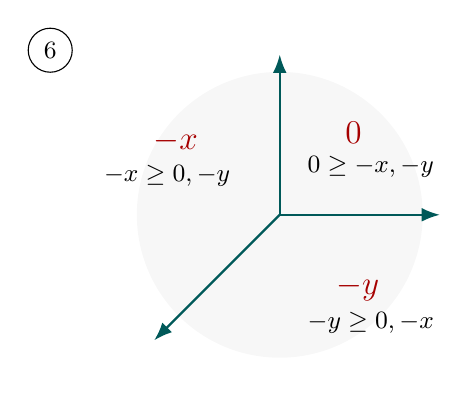
\begin{tikzpicture}[x=1.1cm,y=1.1cm,>=Latex,every node/.style={font=\small}]
    \node[draw,circle,inner sep=3pt] at (-2.65,1.9) {$6$};
    \foreach \start/\sweep in {0/90,90/135,225/135} {
        \path[fill=gray!6,draw=none]
            (0,0) -- (\start:1.65)
            arc[start angle=\start,delta angle=\sweep,radius=1.65] -- cycle;
    }
    \draw[->,thick,teal!70!black] (0,0) -- (1.85,0);
    \draw[->,thick,teal!70!black] (0,0) -- (0,1.85);
    \draw[->,thick,teal!70!black] (0,0) -- (-1.45,-1.45);
    \node[font=\large,text=red!65!black] at (0.85,0.95) {$0$};
    \node at (1.05,0.55) {$0\geq -x,-y$};
    \node[font=\large,text=red!65!black] at (-1.2,0.85) {$-x$};
    \node at (-1.3,0.45) {$-x\geq0,-y$};
    \node[font=\large,text=red!65!black] at (0.9,-0.85) {$-y$};
    \node at (1.05,-1.25) {$-y\geq0,-x$};
\end{tikzpicture}

{\small The active linear function on each cone.}
\end{center}

\section{Ample divisors and toric varieties from polytopes}

With the support-function convention used above, the conclusion of
the previous discussion is
\[
    \boxed{D\text{ is basepoint free}
    \quad\Longleftrightarrow\quad \psi_D\text{ is convex}.}
\]
We now turn to ampleness and very ampleness. This also answers Ayo's
question: \emph{If we start with a lattice polytope, is there a natural
toric variety associated to it?}

\subsection{The trapezoid and its monomial map}

Work over \(\mathbb C\), and consider the trapezoid
\[
    P=\operatorname{conv}\{(0,0),(2,0),(1,1),(0,1)\}
      \subset M_\bR.
\]
Its five lattice points, in the order we will use for homogeneous
coordinates, are
\[
    m_0=(0,0),\quad m_1=(1,0),\quad m_2=(0,1),\quad
    m_3=(2,0),\quad m_4=(1,1).
\]

\Needspace{5cm}
\begin{center}
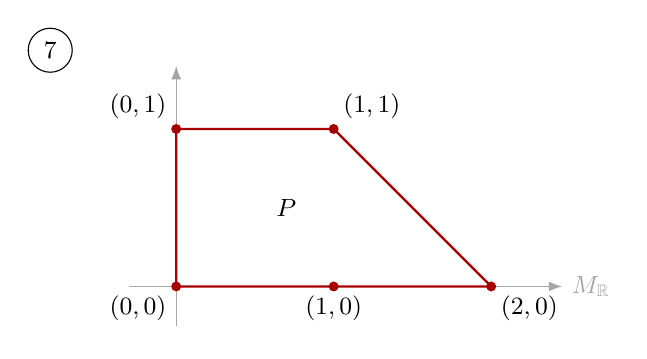
\begin{tikzpicture}[x=2cm,y=2cm,>=Latex,every node/.style={font=\small}]
  \node[draw,circle,inner sep=3pt] at (-0.8,1.5) {$7$};
  \draw[->,gray!70] (-0.3,0)--(2.45,0) node[right] {$M_\bR$};
  \draw[->,gray!70] (0,-0.25)--(0,1.4);
  \draw[thick,red!65!black] (0,0)--(2,0)--(1,1)--(0,1)--cycle;
  \foreach \x/\y/\label/\pos in {0/0/{(0,0)}/below left,1/0/{(1,0)}/below,2/0/{(2,0)}/below right,1/1/{(1,1)}/above right,0/1/{(0,1)}/above left}{
    \fill[red!65!black] (\x,\y) circle(1.8pt);
    \node[\pos] at (\x,\y) {$\label$};
  }
  \node at (0.7,0.5) {$P$};
\end{tikzpicture}

{\small The five lattice points of \(P\) give the coordinates
\(1,s,t,s^2,st\).}
\end{center}

The corresponding characters define a monomial map
\[
    \vf_P:T=(\mathbb C^\times)^2\longrightarrow\bP^4,
    \qquad(s,t)\longmapsto[1:s:t:s^2:st].
\]
Let
\[
    Y=\overline{\vf_P(T)}\subseteq\bP^4
\]
be its Zariski closure. What variety is \(Y\)? We identify it by
examining its affine charts.

Write \(U_i=\{x_i\ne0\}\subseteq\bP^4\) and
\(Y_i=Y\cap U_i\). Since every monomial is nonzero on \(T\),
\(\vf_P(T)\) lies in every \(U_i\), and \(Y_i\) is its closure
inside \(U_i\cong\bA^4\). In a normalized coordinate tuple, we list
\(x_j/x_i\) in increasing order of \(j\ne i\).

\subsection{The chart \(U_0\): the vertex \((0,0)\)}

On \(U_0\), use coordinates \(\widetilde{x}_j=x_j/x_0\), for
\(j=1,\ldots,4\). The torus image is
\[
    (\widetilde{x}_1,\widetilde{x}_2,
     \widetilde{x}_3,\widetilde{x}_4)=(s,t,s^2,st).
\]
Its closure is the graph of the polynomial map
\[
    \bA^2\longrightarrow\bA^2,\qquad(s,t)\longmapsto(s^2,st).
\]
Equivalently,
\[
    Y_0=V(\widetilde{x}_3-\widetilde{x}_1^2,
          \widetilde{x}_4-\widetilde{x}_1\widetilde{x}_2)
          \cong\bA^2.
\]
Its coordinate ring is \(\mathbb C[s,t]\), so the character exponents
generate
\[
    \sigma_0^\vee=\operatorname{cone}((1,0),(0,1))\subset M_\bR.
\]
The dual cone \(\sigma_0\subset N_\bR\) is also the first quadrant.
Thus \(Y_0\cong X_{\sigma_0}\).

\Needspace{4.5cm}
\begin{center}
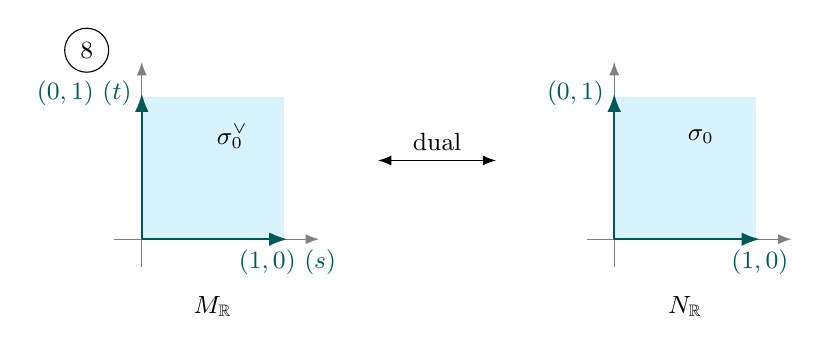
\begin{tikzpicture}[x=1cm,y=1cm,>=Latex,every node/.style={font=\small}]
  \node[draw,circle,inner sep=3pt] at (-0.7,2.4) {$8$};
  \fill[cyan!15] (0,0) rectangle (1.8,1.8);
  \draw[->,gray] (-0.35,0)--(2.25,0);
  \draw[->,gray] (0,-0.35)--(0,2.25);
  \draw[->,thick,teal!70!black] (0,0)--(1.85,0)
    node[below] {$(1,0)\ (s)$};
  \draw[->,thick,teal!70!black] (0,0)--(0,1.85)
    node[left] {$(0,1)\ (t)$};
  \node at (1.15,1.3) {$\sigma_0^\vee$};
  \node at (0.9,-0.85) {$M_\bR$};
  \draw[<->] (3,1)--(4.5,1) node[midway,above] {dual};
  \begin{scope}[xshift=6cm]
    \fill[cyan!15] (0,0) rectangle (1.8,1.8);
    \draw[->,gray] (-0.35,0)--(2.25,0);
    \draw[->,gray] (0,-0.35)--(0,2.25);
    \draw[->,thick,teal!70!black] (0,0)--(1.85,0) node[below] {$(1,0)$};
    \draw[->,thick,teal!70!black] (0,0)--(0,1.85) node[left] {$(0,1)$};
    \node at (1.1,1.3) {$\sigma_0$};
    \node at (0.9,-0.85) {$N_\bR$};
  \end{scope}
\end{tikzpicture}

{\small The chart associated with \((0,0)\) is
\(X_{\sigma_0}=\Spec\mathbb C[s,t]\cong\bA^2\).}
\end{center}

\subsection{The chart \(U_2\): the vertex \((0,1)\)}

Now normalize by \(x_2\), and write \(\widehat{x}_j=x_j/x_2\).
The torus image in this chart is
\[
    (\widehat{x}_0,\widehat{x}_1,
     \widehat{x}_3,\widehat{x}_4)
    =\left(\frac1t,\frac{s}{t},\frac{s^2}{t},s\right).
\]
Set \(u=s\) and \(v=t^{-1}\). The tuple becomes
\[
    (v,uv,u^2v,u).
\]
The first and last entries recover \(v,u\), and the middle entries
are polynomial functions of them. Its closure is therefore another
graph isomorphic to \(\bA^2\), with coordinate ring
\(\mathbb C[s,t^{-1}]\). Hence
\[
    \sigma_2^\vee=\operatorname{cone}((1,0),(0,-1)),\qquad
    \sigma_2=\operatorname{cone}((1,0),(0,-1)),
\]
and \(Y_2\cong X_{\sigma_2}\) is the chart of the fourth-quadrant cone.

\Needspace{4.5cm}
\begin{center}
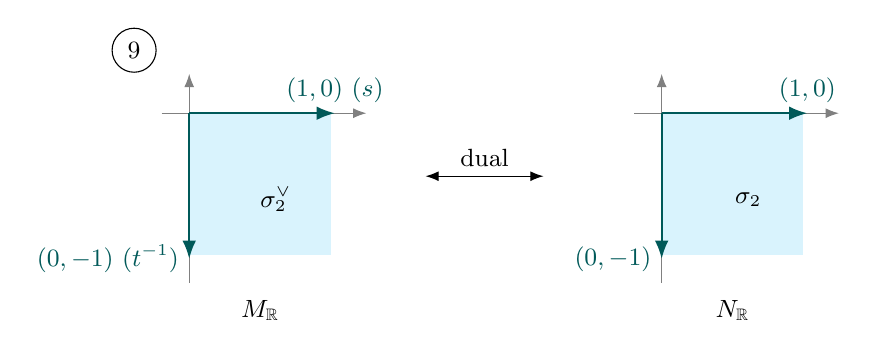
\begin{tikzpicture}[x=1cm,y=1cm,>=Latex,every node/.style={font=\small}]
  \node[draw,circle,inner sep=3pt] at (-0.7,0.8) {$9$};
  \fill[cyan!15] (0,0) rectangle (1.8,-1.8);
  \draw[->,gray] (-0.35,0)--(2.25,0);
  \draw[->,gray] (0,-2.15)--(0,0.5);
  \draw[->,thick,teal!70!black] (0,0)--(1.85,0)
    node[above] {$(1,0)\ (s)$};
  \draw[->,thick,teal!70!black] (0,0)--(0,-1.85)
    node[left] {$(0,-1)\ (t^{-1})$};
  \node at (1.1,-1.1) {$\sigma_2^\vee$};
  \node at (0.9,-2.5) {$M_\bR$};
  \draw[<->] (3,-0.8)--(4.5,-0.8) node[midway,above] {dual};
  \begin{scope}[xshift=6cm]
    \fill[cyan!15] (0,0) rectangle (1.8,-1.8);
    \draw[->,gray] (-0.35,0)--(2.25,0);
    \draw[->,gray] (0,-2.15)--(0,0.5);
    \draw[->,thick,teal!70!black] (0,0)--(1.85,0) node[above] {$(1,0)$};
    \draw[->,thick,teal!70!black] (0,0)--(0,-1.85) node[left] {$(0,-1)$};
    \node at (1.1,-1.1) {$\sigma_2$};
    \node at (0.9,-2.5) {$N_\bR$};
  \end{scope}
\end{tikzpicture}

{\small The chart associated with \((0,1)\) is
\(X_{\sigma_2}=\Spec\mathbb C[t^{-1},s]\cong\bA^2\).}
\end{center}

\subsection{The remaining vertex charts}

The same calculation works at \((2,0)\) and \((1,1)\):
\[
\begin{array}{c|c|c}
    \text{chart and vertex} & \text{parameters} & \text{normalized image}\\ \hline
    U_3,\ (2,0) & u=s^{-1},\ v=t/s & (u^2,u,uv,v)\\[2pt]
    U_4,\ (1,1) & u=s^{-1},\ v=s/t & (u^2v,uv,u,v)
\end{array}
\]
In each row, two entries are \(u,v\), and the others are polynomial
functions of them. The closures \(Y_3,Y_4\) are therefore both
isomorphic to \(\bA^2\). Their cones are
\[
\begin{aligned}
    \sigma_3^\vee&=\operatorname{cone}((-1,0),(-1,1)),
    &\sigma_3&=\operatorname{cone}((0,1),(-1,-1)),\\
    \sigma_4^\vee&=\operatorname{cone}((-1,0),(1,-1)),
    &\sigma_4&=\operatorname{cone}((-1,-1),(0,-1)).
\end{aligned}
\]
Thus \((2,0)\) gives the upper-left cone, and \((1,1)\) gives the
narrow lower cone in the final fan.

The nonvertex lattice point \((1,0)\) gives a different kind of chart.
On \(U_1\), put \(u=s\) and \(v=t/s\). The coordinate tuple is
\[
    \left(\frac1s,\frac ts,s,t\right)=(u^{-1},v,u,uv),
\]
so
\[
    Y_1\cong\Spec\mathbb C[u,u^{-1},v]
        \cong\mathbb C^\times\times\bA^1.
\]
This chart corresponds to the ray \((0,1)\), rather than a maximal
cone. It is not needed in the vertex cover: the relation
\(x_1^2=x_0x_3\), which holds on \(Y\), implies
\(Y_1\subseteq Y_0\cap Y_3\). In particular,
\[
    Y=Y_0\cup Y_2\cup Y_3\cup Y_4.
\]

\subsection{Tangent cones and the normal fan}

At a vertex \(v\), normalizing the coordinate associated with \(v\)
replaces each monomial \(\chi^m\) by \(\chi^{m-v}\). These differences
generate the tangent cone
\[
    \sigma_v^\vee=\operatorname{cone}(P-v)\subset M_\bR.
\]
In this example they generate all its lattice points as a semigroup,
as the two polynomial generators of each vertex chart show. Therefore
the chart is exactly \(X_{\sigma_v}\), where
\[
    \sigma_v=
    \set{u\in N_\bR:\braket{m-v}{u}\geq0\text{ for all }m\in P}.
\]
Equivalently, \(\sigma_v\) consists of linear functionals whose
minimum on \(P\) is attained at \(v\). We use this \emph{inward},
or minimizing, convention for normal cones.

\Needspace{6cm}
\begin{center}
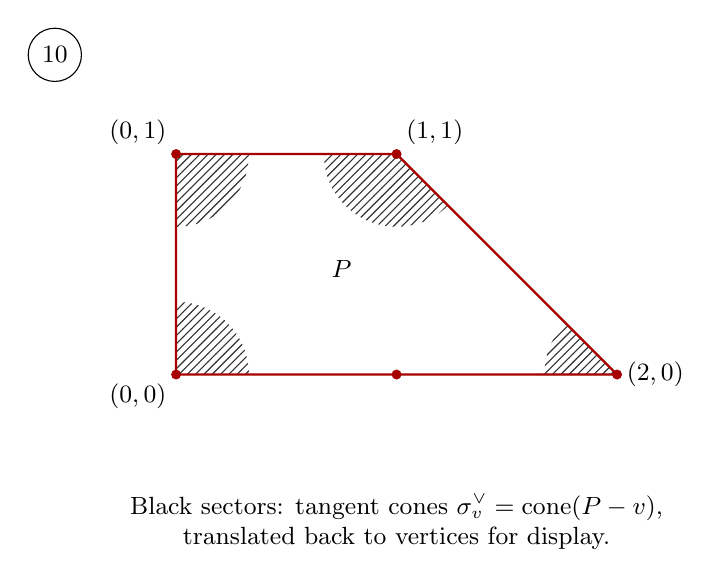
\begin{tikzpicture}[x=2.8cm,y=2.8cm,>=Latex,every node/.style={font=\small}]
  \node[draw,circle,inner sep=3pt] at (-0.55,1.45) {$10$};
  % The shaded angles are tangent cones, not normal cones.
  \foreach \x/\y/\start/\sweep in {0/0/0/90,0/1/270/90,1/1/180/135,2/0/135/45}{
    \begin{scope}[shift={(\x,\y)}]
      \path[pattern=north east lines,pattern color=black!80]
        (0,0)--(\start:0.33)
        arc[start angle=\start,delta angle=\sweep,radius=0.33]--cycle;
      \draw[black!70] (\start:0.37)--(0,0)--({\start+\sweep}:0.37);
    \end{scope}
  }
  \draw[thick,red!65!black] (0,0)--(2,0)--(1,1)--(0,1)--cycle;
  \foreach \x/\y/\label/\pos in {0/0/{(0,0)}/below left,2/0/{(2,0)}/right,1/1/{(1,1)}/above right,0/1/{(0,1)}/above left}{
    \fill[red!65!black] (\x,\y) circle(1.8pt);
    \node[\pos] at (\x,\y) {$\label$};
  }
  \fill[red!65!black] (1,0) circle(1.8pt);
  \node at (0.75,0.48) {$P$};
  \node[below,align=center] at (1,-0.5)
    {Black sectors: tangent cones \(\sigma_v^\vee=\operatorname{cone}(P-v)\),\\translated back to vertices for display.};
\end{tikzpicture}
\end{center}

The four normal cones and all their faces form the normal fan
\(\Sg_P\). Its rays are
\[
    (1,0),\qquad(0,1),\qquad(-1,-1),\qquad(0,-1).
\]

\Needspace{6cm}
\begin{center}
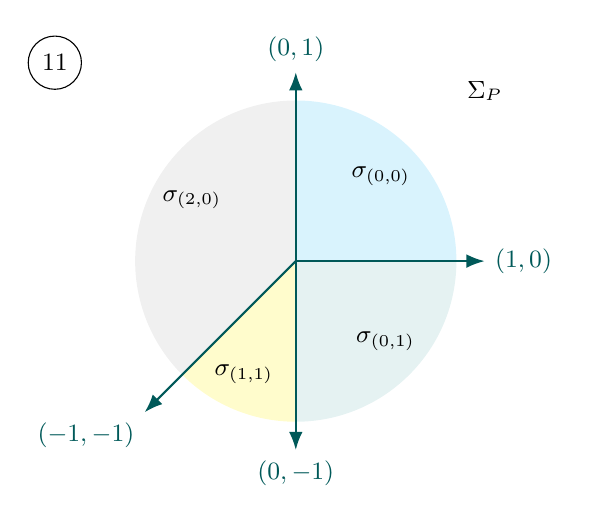
\begin{tikzpicture}[x=1.2cm,y=1.2cm,>=Latex,every node/.style={font=\small}]
  \node[draw,circle,inner sep=3pt] at (-2.55,2.1) {$11$};
  \foreach \start/\sweep/\color in {0/90/cyan!15,90/135/gray!12,225/45/yellow!20,270/90/teal!10}{
    \path[fill=\color] (0,0)--(\start:1.7)
      arc[start angle=\start,delta angle=\sweep,radius=1.7]--cycle;
  }
  \draw[->,thick,teal!70!black] (0,0)--(2,0) node[right] {$(1,0)$};
  \draw[->,thick,teal!70!black] (0,0)--(0,2) node[above] {$(0,1)$};
  \draw[->,thick,teal!70!black] (0,0)--(-1.6,-1.6) node[below left] {$(-1,-1)$};
  \draw[->,thick,teal!70!black] (0,0)--(0,-2) node[below] {$(0,-1)$};
  \node at (0.9,0.9) {$\sigma_{(0,0)}$};
  \node at (-1.1,0.65) {$\sigma_{(2,0)}$};
  \node at (-0.55,-1.2) {$\sigma_{(1,1)}$};
  \node at (0.95,-0.85) {$\sigma_{(0,1)}$};
  \node at (2,1.8) {$\Sigma_P$};
\end{tikzpicture}

{\small The inward normal fan of \(P\): each maximal cone consists
of functionals minimized at the indicated vertex.}
\end{center}

The affine charts glue along the monomial coordinate changes inherited
from the same torus. We have therefore identified the projective closure:
\[
    \boxed{\overline{\vf_P(T)}=Y\cong X_{\Sg_P}.}
\]
This answers Ayo's question: the normal fan is the combinatorial data
of the natural normal toric variety associated to the polytope.

\subsection{The connection with ampleness and very ampleness}

The inequalities for our trapezoid are
\[
    r\geq0,\qquad t\geq0,\qquad t\leq1,\qquad r+t\leq2.
\]
They define a torus-invariant Cartier divisor \(D_P\) on
\(X_{\Sg_P}\) with polytope \(P\). In our support-function convention,
\[
    \psi_{D_P}(x,y)=\max(0,-y,-2x,-x-y).
\]
Its maximal domains of linearity are exactly the maximal cones of
\(\Sg_P\). This is \emph{strict convexity relative to the fan}, the
toric criterion for ampleness. It is stronger than the convexity
criterion for basepoint freeness.

The explicit chart calculations give more in this example: the five
monomial sections identify \(X_{\Sg_P}\) with the closed subvariety
\(Y\subseteq\bP^4\). Hence \(D_P\) is very ample.

\begin{Rmk}
    A full-dimensional lattice polytope always determines a normal fan
    and a normal projective toric variety, together with an ample
    divisor. Identifying this variety with the direct closure of the
    lattice-point map requires an additional check in general; here
    the vertex-chart calculations supply it. For an ample divisor,
    some positive multiple is always very ample.
\end{Rmk}

\end{document}
